
\section{Resultados parciais}

As análise preliminares tiveram um caráter mais exploratório, ou seja, o enfoque foi analisar se os dados dispostos disponham de padrões e tendências esperadas. Dos anos de 1985 até 2021, notou-se uma tendência de crescimento de produção pecuária no estado do Pará, em decorrência disso, é esperado que exista uma correlação entre a área de pastagem e o número de rebanhos. Para podermos confirmar a hipótese, foi gerado um gráfico de correlação de Pearson, que obteve os seguintes resultados: 

\begin{figure}[hbt!]
    \centering
    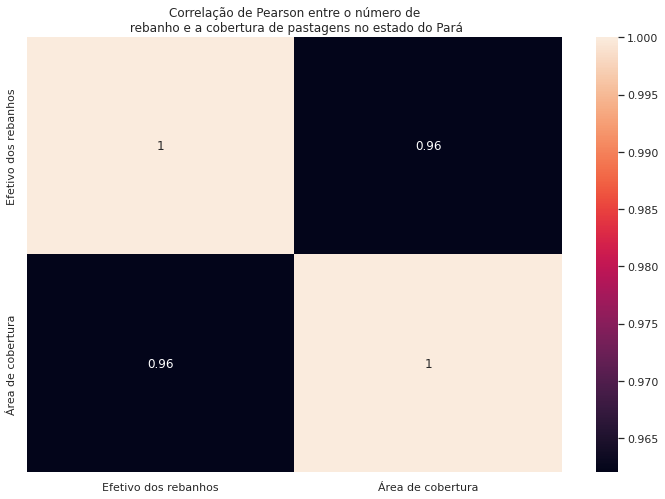
\includegraphics[width=0.7\columnwidth]{src/corr_rebanho_pastagem.png}
    \caption{Correlação entre o número de cabeças de rebanhos em relação a área de cobertura de pastagem no estado do Pará}
    \label{fig:corr_rebanho_pastagem}
\end{figure}

As duas variáveis demonstraram uma alta correlação positiva, o que significa que o crescimento de uma está associada positivamente ao crescimento da outra. Para aprofundar a análise, foi gerado também um gráfico que visa entender o comportamento dos dados ao decorrer dos anos e identificar anomalias e correlações entre eles.
\newpage
\begin{figure}[hbt!]
    \centering
    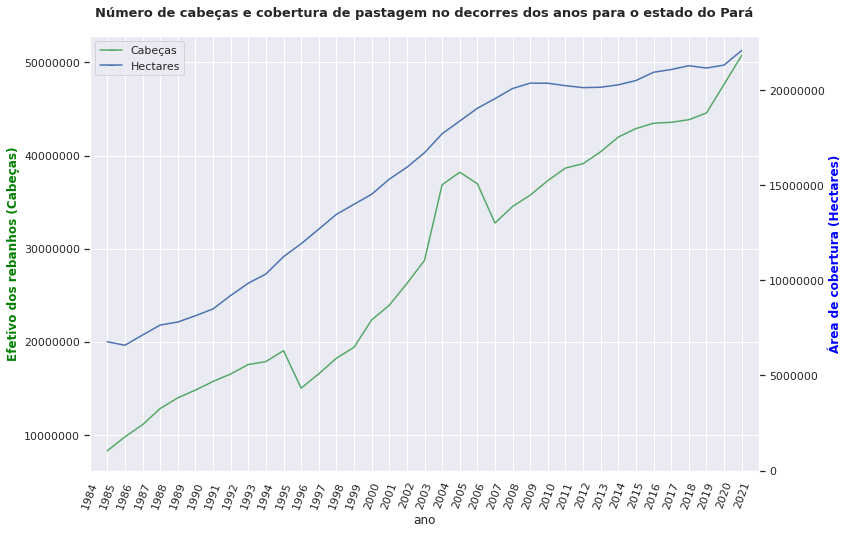
\includegraphics[width=0.9\columnwidth]{src/numero-cabecas-cobertura-pastagem.png}
    \caption{Gráfico temporal de número de cabeças de rebanhos e área de cobertura de pastagem no estado do Pará}
    \label{fig:numero_cabecas_cobertura_pastagem}
\end{figure}

\subsection{Dicionário de dados}